
\documentclass{l4proj}

%Packages
\usepackage{natbib}

\begin{document}
\title{Augmented Reality Android Gym App}
\author{David Benicek 2073063b}
\date{\today}
\maketitle

\begin{abstract}
Something will go here.
\end{abstract}

\educationalconsent
%
%NOTE: if you include the educationalconsent (above) and your project is graded an A then
%      it may be entered in the CS Hall of Fame
%
\tableofcontents
%==============================================================================

\chapter{Introduction}
\pagenumbering{arabic}
\section{Motivation}
Frequent exercise and a healthy lifestyle have recently become an integral part of the western culture. Indeed, last year in America more people have exercised on a regular basis then ever before \cite{USexercise}. As people begin to adopt this new lifestyle it is immediately obvious that there are two distinct periods during which there seems to be a lack of coherent information. These are at the very beginning when a person begins to exercise for the first time and when a person begins to plateau and starts to experience diminishing returns for their work due to a lack of variation in their routine. It is important to note that a lack of coherent information does not necessarily mean a lack of data but instead a lack of singular consensus in the midst of conflicting and misleading information filled with fad diets, ill-informed advice and 'bro science'. It is therefore obvious that there is a need for a singular portal to which beginners and experienced gym goers alike can refer to for information. 

\section{Aim}
Tackling the entire topic of fitness in one application would be extremely difficult, if not impossible. Due to this we are going to focus on the gym environment and look to add value to users while they are in the gym. The aim of the application will be to help users to understand how to use gym equipment, suggest a range of exercises that can be carried out on a given piece of equipment and demonstrate how to perform the exercise with correct and safe form. 

One of the main goals of the app is for it to be responsive to the users environment and heavily interactive so that the user has an immersive experience. However, there is a balance to be struck to ensure that users do not loose awareness of their surrounding. One possible way of achieving this is through augmented reality which will allow us to super impose realistic human models on their device's screen without the need for a completely virtualized reality.  


\section{Outline}
In this document we are going to explore the different steps taken in the development of the augmented reality gym app. First we will look at requirements gathering and elicitation. Then we will discuss the possible designs of the app both from a user experience and user interface aspect. Later we will go trough the steps in implementation and testing, outlining the procedure and any major problems along the way. Finally we will draw the document to a close with a conclusion, followed by an evaluation where we will address to what extend the main goals of the project were achieved and reflect on what could have been done differently for future reference. 

\chapter{Requirements}
The quick brown fox jumped over the lazy dog.
The quick brown fox jumped over the lazy dog.
The quick brown fox jumped over the lazy dog.
The quick brown fox jumped over the lazy dog.

\section{Requirements gathering}
The quick brown fox jumped over the lazy dog.
The quick brown fox jumped over the lazy dog.
The quick brown fox jumped over the lazy dog.
The quick brown fox jumped over the lazy dog.
\subsection{Questionnaire}
The quick brown fox jumped over the lazy dog.
The quick brown fox jumped over the lazy dog.
The quick brown fox jumped over the lazy dog.
The quick brown fox jumped over the lazy dog.
\subsection{Meeting with GUSA}
The quick brown fox jumped over the lazy dog.
The quick brown fox jumped over the lazy dog.
The quick brown fox jumped over the lazy dog.
The quick brown fox jumped over the lazy dog.

\chapter{Design}
\section{User Experience}
The quick brown fox jumped over the lazy dog.
The quick brown fox jumped over the lazy dog.
The quick brown fox jumped over the lazy dog.
The quick brown fox jumped over the lazy dog.
\section{User Interface}
The quick brown fox jumped over the lazy dog.
The quick brown fox jumped over the lazy dog.
The quick brown fox jumped over the lazy dog.
The quick brown fox jumped over the lazy dog.

\chapter{Implementation}
\chapter{Testing}

\chapter{Conclusion}

\chapter{Evaluation}

%\vspace{-7mm}
\begin{figure}
\centering
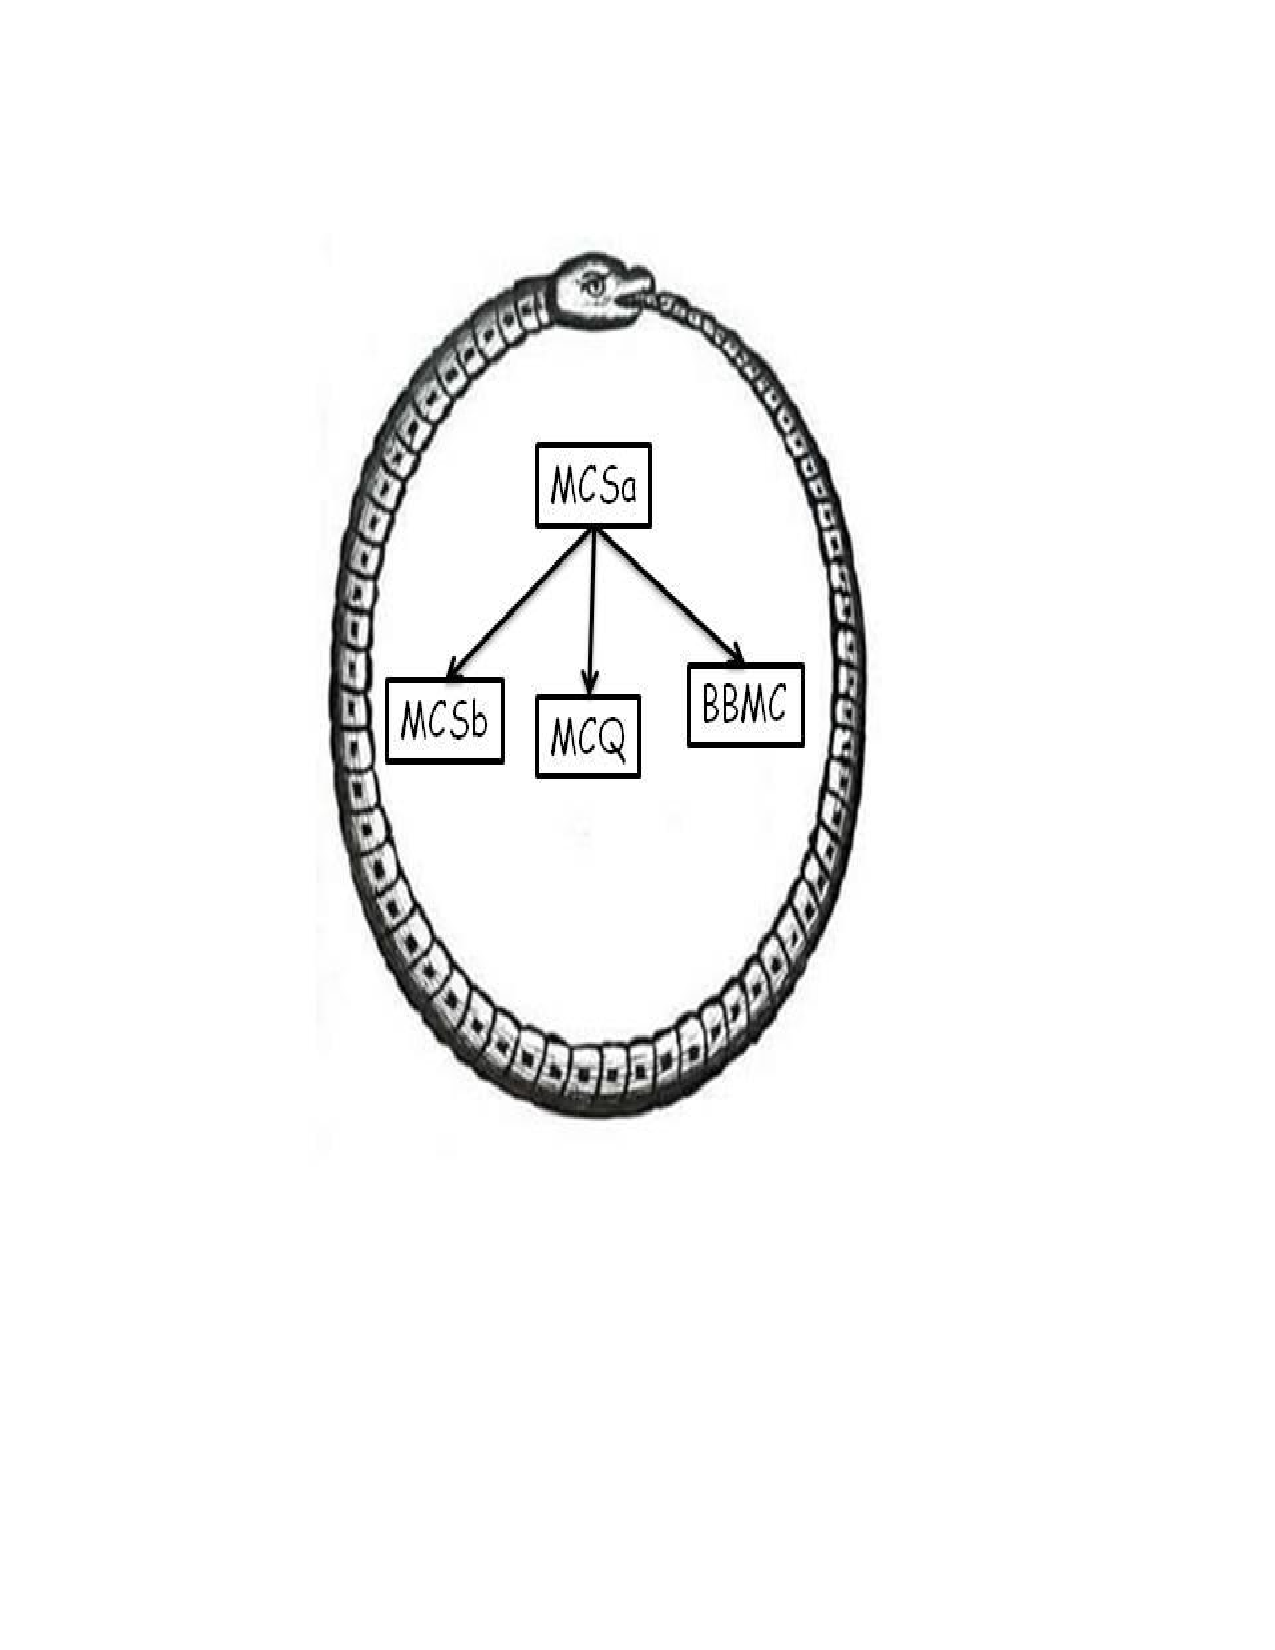
\includegraphics[height=9.2cm,width=13.2cm]{uroboros.pdf}
\vspace{-30mm}
\caption{An alternative hierarchy of the algorithms.}
\label{uroborus}
\end{figure}



%%%%%%%%%%%%%%%%
%              %
%  APPENDICES  %
%              %
%%%%%%%%%%%%%%%%
\begin{appendices}

\chapter{Running the Programs}
An example of running from the command line is as follows:
\begin{verbatim}
      > java MaxClique BBMC1 brock200_1.clq 14400
\end{verbatim}
This will apply $BBMC$ with $style = 1$ to the first brock200 DIMACS instance allowing 14400 seconds of cpu time.

\chapter{Generating Random Graphs}
\label{sec:randomGraph}
We generate Erd\'{o}s-R\"{e}nyi random graphs $G(n,p)$ where $n$ is the number of vertices and
each edge is included in the graph with probability $p$ independent from every other edge. It produces
a random graph in DIMACS format with vertices numbered 1 to $n$ inclusive. It can be run from the command line as follows to produce 
a clq file
\begin{verbatim}
      > java RandomGraph 100 0.9 > 100-90-00.clq
\end{verbatim}
\end{appendices}

%%%%%%%%%%%%%%%%%%%%
%   BIBLIOGRAPHY   %
%%%%%%%%%%%%%%%%%%%%

\bibliographystyle{plain}
\bibliography{bib}

\end{document}
